
\section{Análisis y diseño (SAD)}

La arquitectura del software no es algo unidimensional, sino que esta formado 
por múltiples vistas, como se puede ver en la figura~\ref{fig:sad}, con el 
fin de detallar la funcionalidad, organización y topología del sistema.

\begin{figure}[hp]
	\centering
	\includegraphics[width=10cm]{images/sad.png}
	\caption{Vista de la arquitectura software}
	\label{fig:sad}
\end{figure}

\begin{itemize}
  \item \textbf{Vista de casos de uso:} amplía la representación gráfica 
	de los escenarios descritos durante la especificaciones de casos 
	de uso, definiendo así el comportamiento del sistema en términos 
	funcionales.
  \item \textbf{Vista lógica:} se muestran los requisitos funcionales 
	del sistema. La arquitectura lógica se captura en diagramas de clases 
	que contienen clases y relaciones, para representar las abstracciones 
	clave del sistema en desarrollo.
  \item \textbf{Vista de proceso:} muestra las interacciones en tiempo real de
	los distintos componentes del sistema software, teniendo en cuenta
	requisitos no tenidos en cuenta en otras fases: el rendimiento, la 
	fiabilidad, escalabilidad, integridad, organización del sistema y 
	sincronización. 
  \item \textbf{Vista de implementación:} descompone el sistema software en
	\emph{paquetes}, teniendo en cuenta aspectos como la organización del 
	software, la reutilización, modularidad, facilidad de desarrollo y 
	restricciones impuestas por los lenguajes de programación y las 
	herramientas usadas en el desarrollo
  \item \textbf{Vista de distribucion:} muestra la topología de la arquitectura
	de manera que sea más comprensible por el equipo de desarrollo.
\end{itemize}


\subsection{Vista de casos de uso}

A partir de los casos de uso descritos en la sección~\ref{sec:casos-uso} y 
en la figura~\ref{fig:uml:casos-uso}, se refinaron para extaer una serie 
de casos de uso:

\begin{itemize}
 \item Parametrizar el sistema
 \item Publicar
 \item Enriquecer los datos
 \item Consular los archivos generados
 \item Consultar la información extra generada
\end{itemize}

Se pasará por tanto a describir cada caso de uso en profundidad mediante diagramas
actividas.

\subsubsection{Parametrizar el sistema}

Este caso de uso representa la labor que el usuario administrador debe realizar 
para configurar correctamente el sistema. En la figura~\ref{fig:uml:parametrizar-sistema}
se puede ver el diagrama de actividad de este caso de uso.

\begin{figure}[H]
 	\centering
	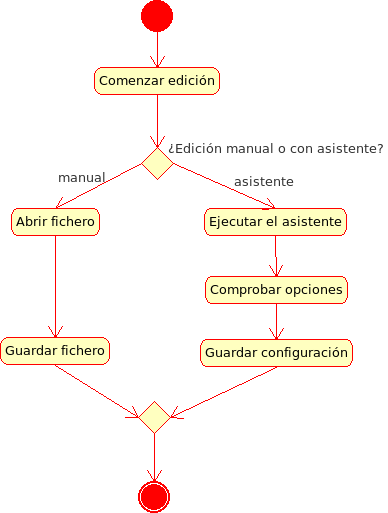
\includegraphics[width=8cm]{images/uml/casos-uso/parametrizar-sistema.png}
	\caption{Diagrama de actividad para el caso de uso «parametrizar el sistema»}
	\label{fig:uml:parametrizar-sistema}
\end{figure}

\subsubsection{Publicar}

Representa la acción de publicación propiamente dicha. El proceso es un proceso por 
lotes que a partir de una configuración genera una serie de ficheros RDF. Internamente
se descompone en varias actividades menores tal y como describe la 
figura~\ref{fig:uml:publicar}.

\begin{enumerate}
 \item \emph{Parsear} el mailbox
 \item Revisar la consistencia de todas las relaciones entre los distintos mensajes
 \item Enriquecer la información
 \item Exportar cada uno de estos mensajes en RDF
 \item Exportar los suscriptores en RDF
 \item Exportar los suscriptores en KML si fuese requerido
 \item Exportar todos los indices
\end{enumerate}

\begin{figure}[H]
 	\centering
	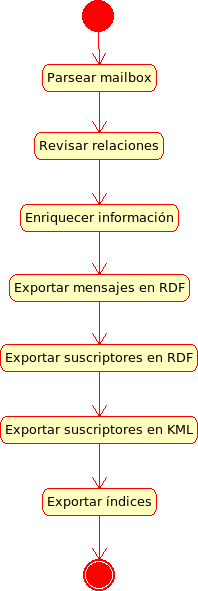
\includegraphics[width=4cm]{images/uml/casos-uso/publicar.png}
	\caption{Diagrama de actividad para el caso de uso «publicar»}
	\label{fig:uml:publicar}
\end{figure}

\subsubsection{Enriquecer los datos}

Representa la interacción del sistema con otras bases del conocimiento externas, 
principalmente los FOAF de los suscriptores a la lista de correo, para enriquecer 
la información en determinados aspectos.

Para cada suscriptor debe repetirse las tareas representadas en la 
figura~\ref{fig:uml:enriquecer}:

\begin{enumerate}
  \item Buscar su FOAF
  \item Si lo tiene:
	\begin{enumerate}
	  \item	Enlazar al suscriptor con su FOAF
	  \item Consultar sus coordenadas geográficas
	  \item Consultar su foto
	\end{enumerate}
  \item Si no lo tiene continuar con el siguiente suscriptor
\end{enumerate}

\begin{figure}[H]
 	\centering
	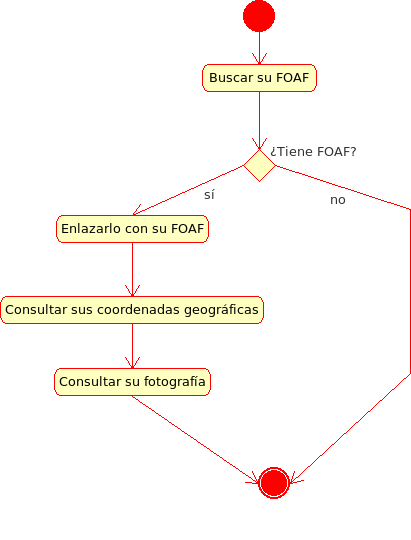
\includegraphics[width=8cm]{images/uml/casos-uso/enriquecer.png}
	\caption{Diagrama de actividad para el caso de uso «enriquecer datos»}
	\label{fig:uml:enriquecer}
\end{figure}

\subsubsection{Consular los archivos generados}

Representa la interacción del usuario con los datos generados. Desde una 
simple consulta manual a los ficheros RDF generados, hasta realizar 
consultas de una forma más sofisticada.

Con la información obtenida se repetirá siempre el mismo flujo descrito en
la figura~\ref{fig:uml:consultar}

\begin{enumerate}
 \item consultar
 \item leer
 \item comprender
 \item y/o desechar
\end{enumerate}

\begin{figure}[H]
 	\centering
	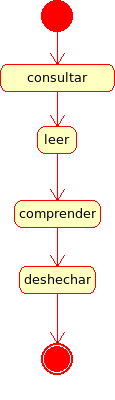
\includegraphics[width=2.5cm]{images/uml/casos-uso/consultar.png}
	\caption{Diagrama de actividad para el caso de uso «consultar»}
	\label{fig:uml:consultar}
\end{figure}

\subsubsection{Consultar la información extra generada}

Este caso de uso representa la consulta por parte del usuario de la 
información extra generada, por el ejemplo los suscriptores en formato 
KML. Las actividades son las que se pueden ver en la 
figura~\ref{fig:uml:consultar-extra}.

\begin{figure}[H]
 	\centering
	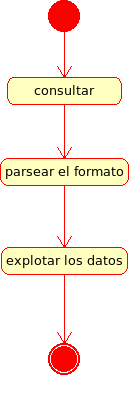
\includegraphics[width=2.5cm]{images/uml/casos-uso/consultar-extra.png}
	\caption{Diagrama de actividad para el caso de uso «consultar información extra»}
	\label{fig:uml:consultar-extra}
\end{figure}




\subsection{Vista lógica}

\subsubsection{Diagrama de clase de SWAML}

\begin{figure}[p]
	\centering
 	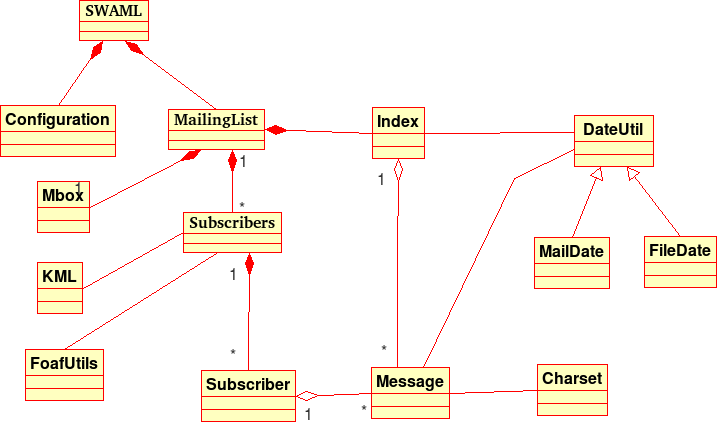
\includegraphics[width=14cm]{images/uml/clases/swaml.png}
	\caption{Diagrama de clase de SWAML}
	\label{fig:uml:swaml}
\end{figure}

\subsubsection{Diagrama de clase de Buxon}

\begin{figure}[p]
	\centering
 	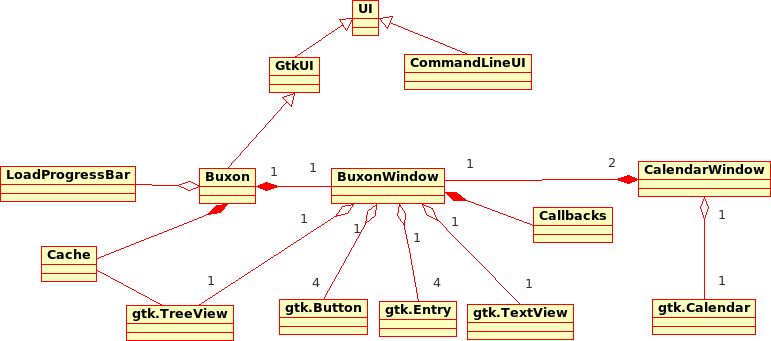
\includegraphics[width=15cm]{images/uml/clases/buxon.png}
	\caption{Diagrama de clase de Buxon}
	\label{fig:uml:buxon}
\end{figure}



\subsection{Vista de proceso}

Se muestran los componentes ejecutables que funcionan en el sistema en 
tiempo de ejecución. El análisis y diseño realizado han dado lugar a 
varios componentes (SWAML, configWizard, Buxon, FOAF Enricher y 
KML Exporter) que interactuan según el diagrama de componentes descrito 
en la figura~\ref{fig:uml:componentes}.

\begin{figure}[H]
	\centering
	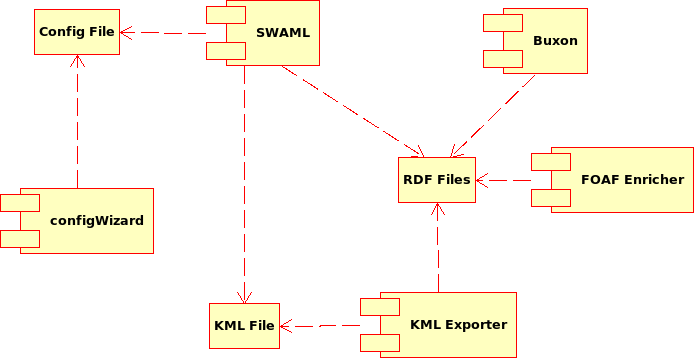
\includegraphics[width=16cm]{images/uml/componentes.png}
	\caption{Diagrama de componentes}
	\label{fig:uml:componentes}
\end{figure}

\subsubsection{SWAML}

Representa el núcleo principal de la aplicación, formado por el script
\texttt{swaml.py}. Implementa toda la lógica de la aplicación para
exportar un mailbox a RDF.

\subsubsection{configWizard}

Mediante el script \texttt{configWizard.py} se provee una forma ágil y 
sencilla de crear los ficheros de configuración que debe recibir SWAML 
como entrada.

\subsubsection{FOAF Enricher}

Representa el medio para enriquecer la información de los suscriptores
usando sus ficheros FOAF con fuente primaria de información.

\subsubsection{KML Exporter}

Mediante este componente se obtiene la información geográfica de los
distintos suscriptores de una lista de correo.

\subsubsection{Buxon}

Representa la interfaz de usuario para visualizar listas de correo
exportadas en SIOC.






\subsection{Vista de implementación}

(describir los paquetes) FIXME



\subsection{Vista de distribución}

FIXME



